\documentclass{report}
\usepackage[utf8]{inputenc}
\usepackage[francais]{babel}
\usepackage[T1]{fontenc}
\usepackage{lmodern}
\usepackage{ifpdf}
\usepackage{graphicx}
\usepackage{geometry}
\usepackage{color}

\definecolor{orange}{rgb}{0.8, 0.4, 0.1}
\definecolor{vert}{rgb}{0.27, 0.57, 0.13}
\definecolor{marron}{rgb}{0.6, 0.2, 0.13}
\renewcommand{\familydefault}{\sfdefault}

\geometry{hmargin=50pt, vmargin=50pt}

\title{Rapport de projet : Moteur de Streaming}
\author{Kevin Bollini \and Thomas Hinsinger \and Valentin Hirson}
\date{\today}
\ifpdf
	\pdfinfo 
	{
		/Author (kbollini,thinsinger)
		/Title (Rapport de projet)
		/Subject (Moteur de Streaming)
		/Keywords ()
		/CreationDate (\today)
	}
\fi

\begin{document}
	% Page de titre
	%\maketitle
	\thispagestyle{empty}
\begin{picture}(40,40)
\put(50,-600){\rule{.2mm}{21cm}}
\put(-50,-70){\rule{20cm}{.2mm}}

\put(70,-50){\textsc{\Huge{Moteur de streaming de monde}}}
\put(360,-100){\textsc{\Large{Rapport de TER}}}

\put(100,-220){\textsc{\large{Kevin Bollini, Thomas Hinsinger, Valentin Hirson}}}

\put(160,-455){
\includegraphics[scale=0.4]{images/logoUM2.jpg}}

\put(230,-530){\textsc{\large{Master informatique}}}
\put(205,-550){\textsc{\large{Année universitaire 2012/2013}}}
\end{picture}
	
	\thispagestyle{empty}
	\newpage
	
	% Sommaire
	\tableofcontents

	%Table des figures
	\listoffigures
	
	\newpage
	%TODO : grossir, centrer sur la page
	\section*{Remerciements}
	\addcontentsline{toc}{section}{Remerciements}
	\paragraph{}
Nous tenons à remercier personnellement Marc Moulis pour nous avoir répondu très rapidement aux questions qui se sont posées à nous et d'avoir pris le temps de faire des réunions hebdomadaires. 
	\part{Rapport de projet}
	\newpage
	\chapter{Introduction}
		\section{Présentation projet}
	
		\paragraph{}Notre équipe de 3 personnes devait développer un moteur de streaming (asynchrone) d'univers en temps réel. C'est à dire qu'à partir d'un fichier contenant les coordonnées des points constituant un monde, nous devions l'afficher via OpenGL ou DirectX. 
Mais avec la contrainte de n'afficher que les objets situés à une certaine distance pour permettre un rendu plus fluide. Nous devions donc nous focaliser sur :
\begin{itemize}
	\item le format de découpe de l'univers 
	\item le format de stockage des données 
	\item le chargement asynchrone des données 
	\item la gestion de la visibilité
	\item l'affichage d'objets polygonaux statiques et dynamiques
	\item la gestion des ressources communes (les textures, les maillages, etc...)
	\item et la gestion des entités ponctuelles (bonus, waypoints)
\end{itemize}

		\begin{figure}[!h]
			\centering
			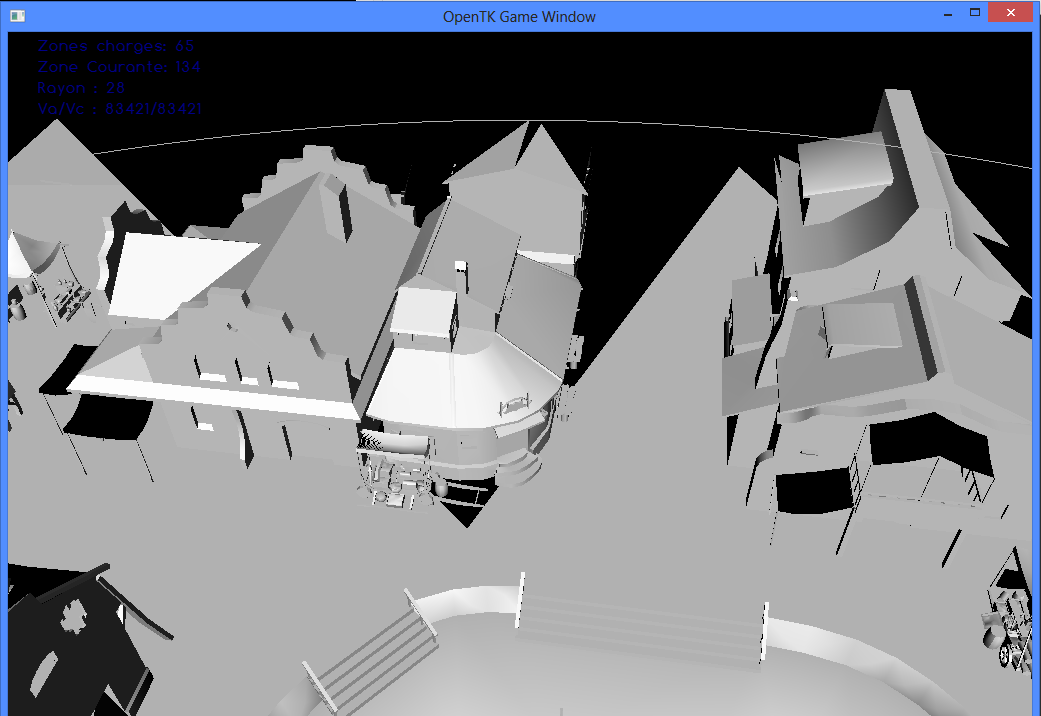
\includegraphics[scale=0.3]{images/capture1.png}\\
			\caption{Aperçu de l'application}
			\label{Aperçu de l'application}
		\end{figure}
		\section{Contexte}
			\paragraph{}La création de ce projet se fait dans la continuité de l'unité d'enseignement "Moteur de jeu 3D" dans le cadre de la deuxième année du Master d'Informatique IMAGINA. Nous avons eu  seulement deux mois pour le mettre en place.  

	\chapter{Analyse et conception}
		\section{Gestion du projet}
			Pour le développement de ce projet, nous avons décidé d'utiliser une méthode AGILE. Nous avons procédé par série de sprints, visant à développer des versions prototypes du moteur puis à les enrichir par itérations successives.\\ \\
		\begin{tabular}{| l | c || r ||}
			 \hline                 
				Version du Prototype & Contenu et Ajouts majeurs & Durée (Jours)\\
			\hline
				1 & Chargement et Rendu non texturé de Scène wavefront  & 3 \\
        					&  Création du projet et du dépôt & \\
			\hline
				2 & Gestion de la Camera, chargement de materials & 2 \\
        					&  Création classe Camera & \\
			\hline
				3 & Zonage de la scène chargée & 2 \\
        					& Modification conception, Ajout classe Zone & \\
			\hline
				4 & Écriture de la scène Zonée dans un fichier propriétaire & 1 \\
        					& Conception du Format maison .zs & \\
			\hline
				5 & Chargement Zone-à-Zone à partir du fichier pré-processé & 1 \\
        					& Création classe AsyncLoadingManager & \\
			\hline
				6 & Mise en Thread du chargement/libération de zones & 2 \\
        					& Création classe AsyncLoadingManager & \\
			\hline
				7 & Mise en place du rayon de charge de Zones & 2 \\
			\hline
				8 & Implémentation du Frustum Culling & 3 \\
			\hline
				9 & Ajouts d'interfaces et de commandes& 2 \\
					& Dessin du rayon de charges, affichage nombre zone chargée& \\
			\hline



 \end{tabular}
\newpage
		\section{Outils utilisés}
			\subsubsection{Outils techniques}
				\begin{itemize}
					\item Integrated Development Environment : Monodevelop
					\item Gestionnaire de version : Subversion
					\item Communication : Mails, outils de vidéoconférence,  éditeur de documents collaboratif
				\end{itemize}
			\subsubsection{Langage :}
				\paragraph{} Après  une étude préalable, nous avons décidé d'utiliser le langage de programmation C\# pour le développement  du projet.
En effet ce choix n'est pas dû au hasard. La principale raison de celui-ci est l'opportunité de découvrir une technologie non traitée au cours de notre formation, dans le cadre d'un projet conséquent.\\ D'autre part, nous avons choisi d'utiliser l'implémentation libre Mono de C\# et de son framework .Net, pour des raisons d'éthique et d'une meilleur portabilité du code sous d'autres OS que Windows.
			\subsubsection{Bibliothèque :}
	\paragraph{OpenTK} est une bibliothèque bas niveau wrappant en C\# OpenGL. Nous avons décidé de l'utiliser car OpenTK  est une des bibliothèques permettant le développement 3D sous C\# les mieux documentées, maintenue et ayant un réel binding objet d'openGL.
			\subsubsection{Format des scènes :}
	\paragraph{Objet3D (.obj créé par la société Wavefront)} Nous avons décidé d'utiliser ce format libre car c'est l'un des formats des plus courants, nous permettant ainsi de récupérer ou modéliser nous mêmes des scènes pour tester notre application. Par ailleurs, c'est un format ouvert et fonctionnant avec beaucoup de logiciels 3D comme Blender, ce qui nous a permis d'avoir un autre aperçu de nos scènes.
		\newpage
		\section{Analyse}		
			\subsection{Diagramme de classes}
				
				%TODO présentation structure \\
				\begin{figure}[!h]
						\centering
						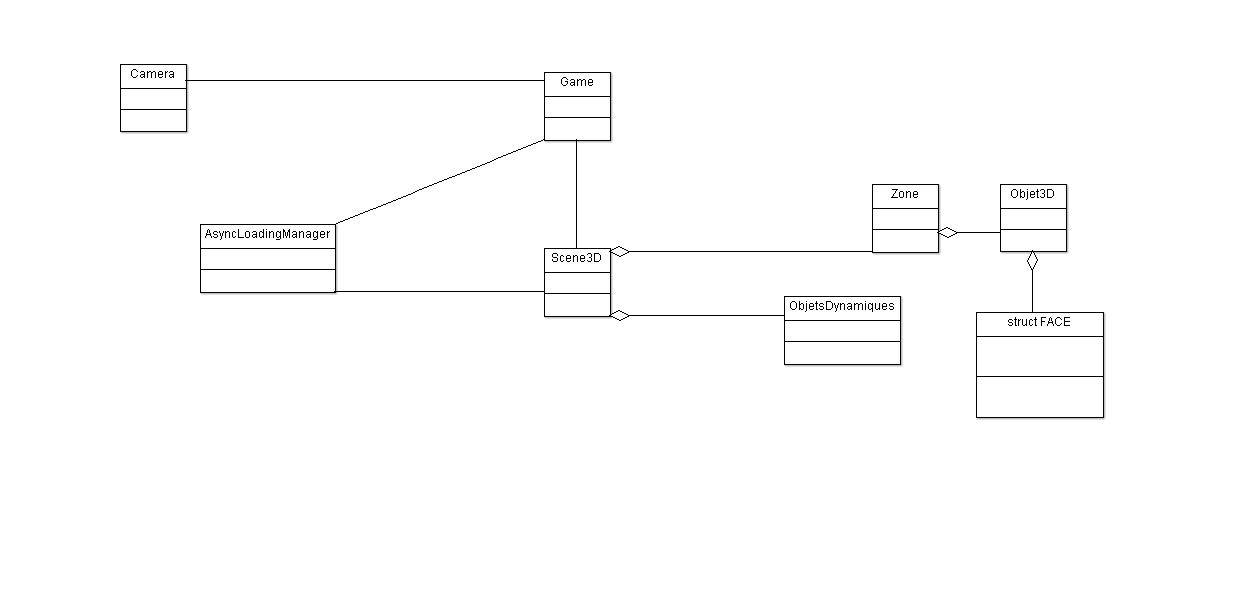
\includegraphics[scale=0.5]{images/ClassDiagram.png}\\
						\caption{Pseudo-Diagramme de classe}
						\label{Pseudo-Diagramme de classe}
				\end{figure}						
	
	\chapter{Réalisation}
		Dans ce chapitre nous détaillerons les points essentiels de notre réalisation en illustrant une partie des composantes développées pour le moteur.
		\section{Préprocessing}
		Dans la phase de conception, nous avons décidés d'utiliser des scènes .obj existantes plutôt que de les générer nous même pour ensuite les streamer. Cela implique donc que nous ayons à effectuer un préprocessing sur les scène avant de pouvoir les exploiter.\\
	Cette étape préliminaire se déroule en trois temps : chargement de la scène, zonage et ré-écriture de la scène.
			\subsection{Chargement de scène Objet3D}
				\paragraph{}
					Avant toutes choses, il nous a fallu comprendre le fonctionnement d'un .obj. Heureusement le format étant ouvert, il nous a été facile de trouver de la documentation dessus. Et le format .obj étant en ASCII, cela a rendu plus facile sa manipulation. \\
Une petite explication du fonctionnement d'un fichier .obj s'impose : un commentaire peut être placé en débutant la ligne par un \# ; Une surface polygonale est décrite par un ensemble de sommets (accompagné de coordonnées de texture et de normales en chaque sommet) et d'un ensemble de faces. Les différentes informations possibles dans un fichier .obj étant assez nombreuses, je ne vais pas toutes les détailler mais je vais détailler les principales et surtout celles que nous avons rencontrées dans les différents fichiers .obj avec lesquels nous avons travaillé (que ce soient ceux générés par Blender ou ceux trouvés sur internet). \\

Un sommet est défini de la manière suivante:

	v 1.0 0.0 0.0 \\

Une coordonnée de texture est définie de la manière suivante:

	vt 1.0 0.0\\


Une normale est définie de la manière suivante:

	vn 0.0 1.0 0.0\\


Chaque face est ensuite définie par un ensemble d'indices faisant référence aux coordonnées des points, de texture et des normales définies précédemment.\\

Par exemple, la face suivante

	f v1/vt1/vn1 v2/vt2/vn2 v3/vt3/vn3\\

définit un triangle constitué des sommets d'indices v1, v2 et v3 dans la liste des sommets v. Chacun de ces sommets possède une coordonnée de texture identifiée par son indice dans la liste des coordonnées de texture vt et une normale identifiée dans la liste des normales vn.

\newpage

Lorsque plusieurs objets cohabitent dans le même fichier, la section définissant l'objet est définie par

o [nom de l'objet]

Lorsque plusieurs groupes de faces cohabitent dans le même objet, la section définissant chaque groupe est définie par

g [nom du groupe]


Des matériaux peuvent être référencés en important des fichiers .mtl (Material Template Library)

usemtl [nom de matériau]

\begin{figure}[!h]
			\centering
			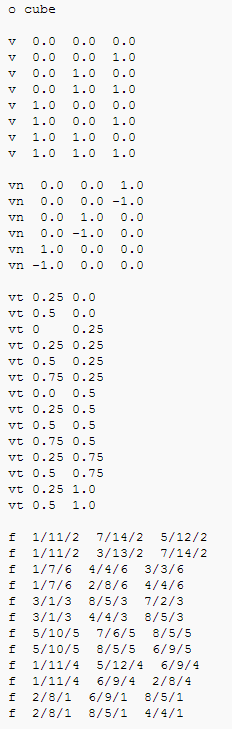
\includegraphics[scale=0.8]{images/exOBJ.png}\\
			\caption{Exemple de .obj}
			\label{Exemple de .obj}
\end{figure}



Nous avons travaillé sur différentes scènes de différentes tailles. Mais pour la présentation du projet, nous nous sommes mis d'accord qu'il fallait une scène 3D suffisamment grande. Après quelques recherches sur internet infructueuses, et quelques essais plus moches les uns que les autres avec Blender, nous avons eu l'idée de voir si on pouvait récupérer une carte d'un jeu vidéo. De fil en aiguille, nous avons trouvé un logiciel (Crafty) permettant de convertir les maps (.bsp) du célèbre jeu Half-Life et de ses extensions en fichier .obj. Par soucis de temps nous n'avons pas pu faire nous même le convertisseur. Le seul soucis c'est que le logiciel n'avait pas été mis à jour depuis 2006, et il n'arrivait pas à récupérer les textures de la carte. Après quelques recherches, et quelques réglages dans fichiers de configuration de Crafty, nous avons réussi à lui indiquer le chemin des textures manquantes et exporter par la même occasion ce qu'il manquait. 
			\newpage	
			\subsection{Zonage}
			\subsubsection{Zonage}
			Il a fallut pour réaliser ce moteur de streaming de monde asynchrone mettre en place un zonage de monde. C'est à dire diviser le monde, qui dans la plus part des temps se trouve beaucoup trop grand pour être afficher en totalité par le moteur physique, en petite zones. Ces zones possèdent ,comme une scène à part entière, un nombre d'objets, de faces, de textures associées.
			
			Avant de décider quel découpage nous allions utiliser il nous a fallu réfléchir un petit peu. Il nous fallait un zonage rapide et efficace. Donc nous avons directement éliminé les découpage de type Octree, Quadtree, etc... Certes cela se fait dans le préprocessing, donc si cela met un peu plus de temps cela n'est pas très grave. Mais après en avoir discuté ensemble avec notre tuteur Marc Moulis, un simple découpage en grille suffisait amplement pour ce qui est du zonage de notre monde.
			
			Voilà à quoi ressemble le zonage : 
			
			 \begin{figure}[!h]
				\centering
					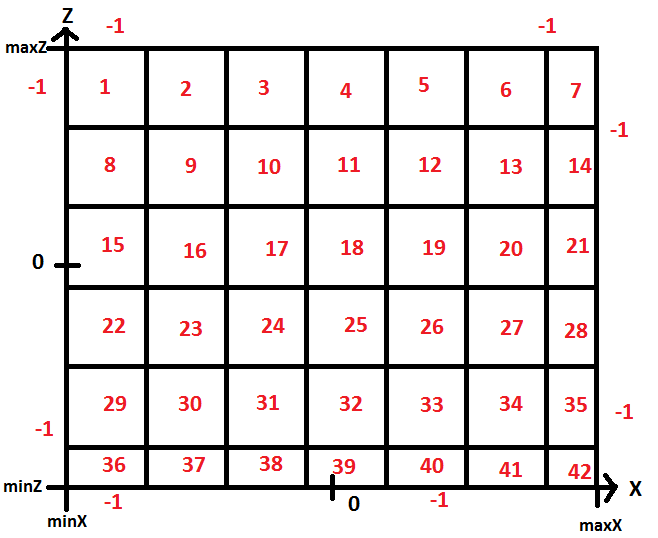
\includegraphics[scale=0.8]{images/zonage.png}\\
					\caption{Zonage de la scène}
					\label{Zonage de la scène}
			\end{figure}	
			
			 Pour construire ce zonage, il faut se servir de données calculées lors du chargement de scène. En effet lorsque l'on parcourt le fichier .obj de la scène que l'on veut charger dans notre moteur de streaming de monde, on regarde toutes les vertex une à une pour trouver les extrémités de notre scène (ce que l'on peut voir sur le schéma ci-dessous "minX, maxX, minZ, maxZ"). De plus on peut découper notre scène selon un paramètre. Ce paramètre définit la largeur et donc la longueur de nos zones (en effet nos zones sont en forme de carré).  Il suffit alors de diviser la largeur de notre scène par ce paramètre pour connaître le nombre de zones sur l'axe X de la scène. De même pour la longueur de notre scène, on la divise par ce paramètre pour connaître le nombre de zones sur l'axe Z. 

			\subsubsection{Position}					

			Il y a une fonction très importante qu'il est nécessaire d'expliquer. Celle-ci permet en fonction d'un Vecteur3 (c'est à dire un point dans l'espace) de situer dans quelle zone ce situe ce point. Et pour réussir à faire ceci c'est très simple. On connait la largeur et la longueur de notre scène. On connait de plus le nombre de zones sur la largeur et la longueur de notre scène. Avec tous ces éléments, il est vraiment facile de connaître le numéro de la zone du point donné en paramètre.																																											
			\subsubsection{Découpage}
			
			Une fois que l'on a zoné notre scène il faut alors découper celle-ci. Quand je dis découper, je dis placer les objets de la scène en fonction du zonage de celle-ci. Imaginons une maison, qui se situe pile entre 2 zones, il faut découper cet objet en deux parties, l'une ira dans une zone, l'autre ira dans la deuxième zone. Cependant il ne faut pas oublier que ces deux sous-objets appartiennent toujours au même objet.
			
			Pour réaliser ceci, tout d'abord il a fallu créer des identifiants à nos objets. Ceci se fait lors de la lecture du fichier .obj. Dès que l'on trouve un nouvel objet on lui associe un ID unique. Pour ce qui est du découpage, c'est très simple. Rappelons toutefois que chaque objet possède un certains nombre de faces. Une fois ceci en tête, il suffit de parcourir la scène entière. Dès que l'on trouve un objet, on parcourt itérativement la liste de ses faces. Ensuite il suffit de repérer dans quelle zone se situe le centre de cette face. Précisons tout de même que le centre de chaque face est calculé lors de la première lecture du fichier .obj. On rajoute cette face dans le sous-objet correspondant à l'objet de la zone. En effet chaque zone possède un objet qui lui est propre. C'est ainsi que le découpage se réalise.
			
			\subsection{Export en format propriétaire}

				\paragraph{}

Tout d'abord expliquons pourquoi avoir eu besoin de créer un format propriétaire. Nous avons eu besoin de découper l'espace en zone pour pouvoir streamer. Nous nous sommes demandé comment fonctionnaient les jeux vidéos, et dans la plupart une barre de chargement 
apparait avant le lancement du jeu. Par ailleurs le format de fichier .obj ne contient pas d'informations sur d'éventuelles zones ou sous zones. Nous nous sommes donc inspirés des jeux vidéos et avons décidé de stocker les informations que nous aurions besoin dans un fichier crée par nous.\\
				 
Les avantages d'un tel système, c'est que l'on peut mettre les informations que l'on juge utiles. Une alternative aurait été de rester sur un format .obj et d'y ajouter en commentaire les informations que l'on aurait besoin. Mais la création d'un format propriétaire nous semblait plus intéressante à mettre en place.\\

				
Par contre, l'inconvénient principal, c'est que l'on doit passer par une phase de préprocessing (chargement) avant de pouvoir faire fonctionner le streaming puisque l'on doit générer le fichier propriétaire avant de faire le rendu.\\

				En pratique cela se traduit par l'utilisation d'un flux pour écrire dans un fichier ASCII. On récupère un objet Scene3D contenant les coordonnées des différents objets de la scène, les informations de texture, etc puis on écrit ces informations dans un fichier portant l'extension .zs.\\

On en vient maintenant à l'explication du format :\\
\begin{itemize}
	\item  \# permet l'écriture de commentaire
	\item  b <xMin> <xMax> <zMin> <zMax> sont les limites
	\item v <index> <X> <Y> <Z> la position dans l'espace d'un sommet d'une face
	\item vt <index> <X> <Y> <Z> les coordonnées des textures
	\item vn <index> <X> <Y> <Z> les coordonées des normales
	\item face : f <vX/vtX/vnX> <vY/vtY/vnY> <vZ/vtZ/vnZ>
	\item z <index> <name> Tous les points situés en dessous de cette ligne font partis de la zone "name"
	\item\item o <centerX> <centerY> <centerZ> les coordonnées du centre de l'objet.
\end{itemize}
				Le seul problème que nous ayons rencontré, était un problème de conception. Lorsque nous avons réussi à convertir en .obj  la map de\_dust.bsp provenant d'un célèbre jeu vidéo. Nous nous sommes aperçu que nous ne gérions pas les faces à plus de 3 sommets. (Nous ne travaillions alors qu'avec des triangles). Il a fallu faire quelques modifications pour pouvoir gérer les faces à n sommets.

		\newpage			

		\section{Chargement Asynchrone}
			La principale problématique du projet est évidement le chargement asynchrone des ressources de la scène. Or qui dit chargement, dit stockage. 
			\subsection{Stockage des données}
			On peut distinguer plusieurs types de ressources nécessitant un traitement différent pour leur stockage.
			\begin{itemize}
				\item éléments statiques : Décors, terrain, etc.
				\item éléments dynamiques : Acteurs, Power-ups, etc.
				\item Textures et Materials
			\end{itemize}
			La différence de traitement réside en le fait qu'un objet dynamique ne sera pas découpé comme on l'a vu dans le point précédent, et que d'autre part, le modèle d'un objet dynamique et les textures peuvent être utilisés plusieurs fois dans la scène. On doit alors gérer ce partage de ressource pour ne pas allouer plusieurs fois une même ressource ou la dés-allouer trop tôt.
			\subsubsection{Statiques}
				Les éléments statiques sont regroupés dans des entités Zone. Une zone contient une liste d'Objet3D, qui elle-même contient des faces. Les différentes vertex de la scène sont elles toutes stockées à la racine de la scène, ceci permettant de partager entre les zones les vertex pouvant appartenir à plusieurs entités ou zone distincte.
			\subsubsection{Dynamiques}
				Les éléments dynamiques doivent être gérés différemment. En effet, les objets dynamique, comme un power-up ou une voiture	 sont des éléments qui peuvent et qui sont souvent utilisés plusieurs fois. La problématique est donc de ne charger leur modèle qu'une seule fois, et ensuite de surveiller leur nombre d'utilisation pour pouvoir les charger ou décharger au moment les plus opportuns.
			\subsubsection{Textures et Materials}
			La problématique pour les textures et materials est sensiblement la même que pour les objets dynamiques. Il serait mal venu d'avoir en mémoire plusieurs fois la même chose, il faut donc ne les charger qu'une fois et de comptabiliser leur nombre d'utilisateurs, de manière à ne les décharger que si ils deviennent obsolètes.

		\subsection{Tâches de chargement/libération}
			On parle ici de chargement asynchrone, ce qui veut dire que les données nécessaires sont chargées à l'exécution en fonction du contexte. Or, il ne faut cependant pas interrompre le rendu pour effectuer la récupération ou libération des données. Nous avons donc décidé d'effectuer ces tâches par le biais d'un thread secondaire dans la classe AsyncLoadingManager.\\

Cette tâches ne s'occupe que de charger ou décharger des données en fonction de tâches que la boucle principale lui donne.
			\subsubsection{Chargement de zone}
				La classe fonctionne avec une pile de tâche à accomplir, nous utilisons une pile de manière à avoir un fonctionnement LIFO (Last In First Out), permettant de traiter toujours les tâches les plus récentes en premier. L'interaction avec ce thread ne se fait que par cette pile, on ajoute une tâche à la pile, et celle-ci sera traitée dès que possible.
				Le traitement est ensuite assez trivial, on regarde dans la scène actuelle si une zone donnée à chargée l'est ou non, si elle ne l'est pas, on va la récupérer dans le fichier, et on l'ajoute à la liste de zone chargée.
			\subsubsection{Libération de zone}
			La libération d'une zone est moins triviale que nous pourrions l'imaginer. En effet, il ne suffit pas de la supprimer de la liste de zones, il faut d'abord parcourir en intégralité cette zone, et de réduire de un le nombre d'utilisateur de chaque texture, material et toute donnée partagée avant de supprimer la zone.
Il faut aussi penser à supprimer de la mémoire chacun de ses items si leur nombre d'utilisateurs tombe à zéro.
\newpage				
		\section{Rendu}
		\subsection{Calcul des zones}
			Pour ce qui est du rendu des zones chargées, il a fallu mettre en place une fonction permettant en fonction d'un radius de définir le nombre de zones qui doivent être affichées à l'écran et d'envoyer ceci au AsyncLoadingManager qui se chargera de la synchronisation du chargement et déchargement des zones. Voici le schéma permettant de comprendre l'exécution de cette fonction : 
			
			\begin{figure}[!h]
				\centering
				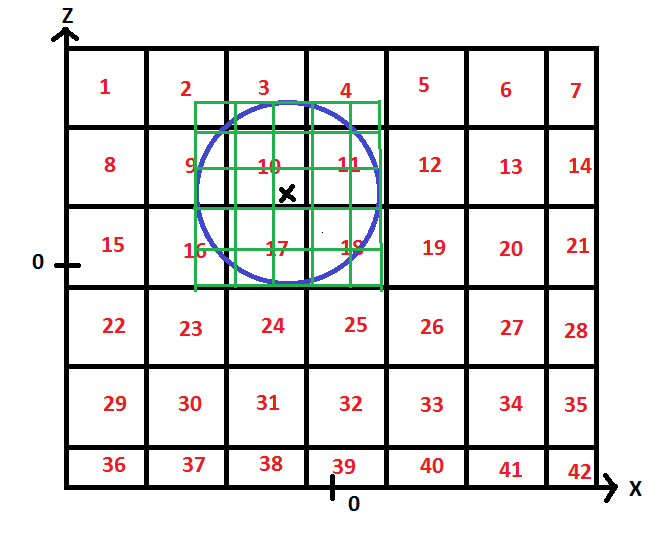
\includegraphics[scale=0.8]{images/calculZone.png}\\
				\caption{Exemple de calcul des zones à afficher.}
				\label{Calcul Zone}
			\end{figure}
			
			Pour comprendre cette fonction il faut identifier dans un premier temps le cercle bleu sur le schéma ci dessus. Toutes les zones se trouvant à l'intérieur de ce cercle doivent être affiché. On repère aussi sur ce schéma un quadrillage vert. Au démarrage de la fonction, on place un point temporaire se situant à X - rayon et à Z - rayon. En effet cette fonction prend en paramètre le rayon dans lequel le nombre de zone doivent s'afficher. On se retrouve donc en haut a gauche du quadrillage vert sur le schéma. On vérifie alors si cette zone est dans le cercle, si c'est le cas, on la rajoute dans la liste de zone à afficher. Et itérativement on va regarder chaque case du quadrillage pour vérifier s'il appartient au cercle.
			
			\subsection{Frustum Culling}
			Une fois que l'on a notre chargement asyncrone de données, c'est bien mais ce n'est pas suffisant. En effet, nous avons un gain de performance assez énorme en évitant de charger une scène énorme en mémoire et en l'affichant. Le moteur physique en prend un sacré coup. Mais il faut aussi se rappeler une chose : Si la caméra se situe en un point et regarde dans une direction dans une zone x de la scène. Le moteur physique va alors afficher a l'écran entièrement la zone x. Il y a donc un certain nombre de points, qui sont dessinés à l'écran mais que le caméra ne peut pas voir. Pour gagner encore plus en performance il faut alors appliquer à notre affichage un Frustum Culling. Regardons comment ça marche : 
			
			\begin{figure}[!h]
				\centering
				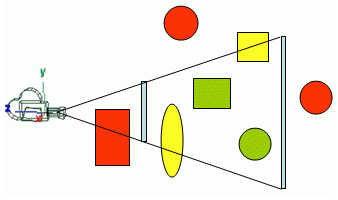
\includegraphics[scale = 1.2]{images/culling.png}\\
				\caption{Frustum Culling}
				\label{Frustum Culling}
			\end{figure}		
			
			En vert, on a les objets que l'on doit entièrement afficher, en jaune les objets qui doivent s'afficher partiellement, et en rouge les objets qui ne doivent pas du tout s'afficher.
			
			Il faut donc avant de pouvoir définir si un objet puisse s'afficher ou non (je dis objet mais il faut plutôt préciser que l'on parle ici de points et non d'objets) il faut donc calculer tous les plans de notre Frustum Culling : 
			
			\begin{figure}[!h]
				\centering
				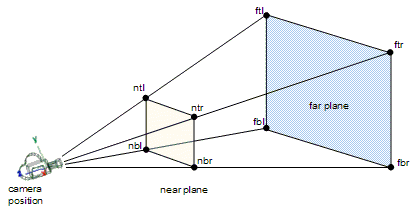
\includegraphics[scale=1.2]{images/plans.png}\\
				\caption{Les différents plans du Frustum Culling}
				\label{plans}
			\end{figure}
			
			Dans un premier temps il est donc nécessaire de calculer les 8 points qui délimiteront les extrémités des six plans de notre Frustum Culling. Pour réussir à faire ceci il faut : 
			
			\begin{figure}[!h]
				\centering
				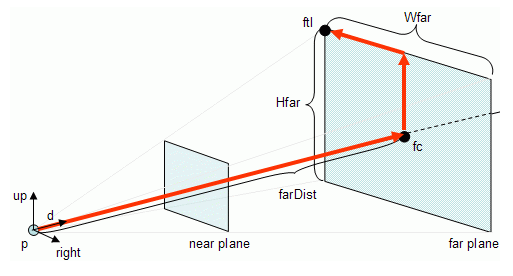
\includegraphics[scale=0.9]{images/pointsPlans.png}\\
				\caption{Exemple de calcul du points ftl}
				\label{calcul point}
			\end{figure}
			
			Une fois que toutes les extrémités sont calculées on peut alors calculer les six plans de notre Frustum Culling.
			
			Ensuite il est facile de savoir si un point se situe ou non à l'intérieur ou non de notre Frustum Culling. Il suffit alors lors du chargement de notre zone et de l'affichage de celle-ci, de vérifier si un point se situe ou non dans le Frustum Culling et si tel est le cas afficher ce point.
																						
			Il faut préciser que dans notre cas on à simplifier au maximum le Frustum Culling, et on affiche non pas point à point mais face à face. Donc le Frustum Culling doit décider si une face doit être affichée ou non. On a décidé que si un point de la face se situait dans le Frustum Culling, la face tout entière devait être affichée. Cependant cela peut poser problème car si par exemple les trois points de la face se situent tous les trois en dehors du Frustum Culling, mais que cette face passe par le Frustum Culling, cette face ne sera pas affichée. C'est une des perspectives d'amélioration de notre Frustum Culling, améliorer celui-ci.																

	\chapter{Discussion}
		\section{Difficultées rencontrées}
			\paragraph{Synchronisation}
				Le principal frein que nous avons rencontré dans ce projet est la synchronisation. En effet, nous ne nous connaissions pas tous avant le projet, et venions d'horizons différents.
				La majeur difficulté apportée par cela est que nous n'avons pas pu pleinement exploiter le temps nous étant imparti, l'un des membres ayant une activité professionnelle à assurer en plus du projet.
			\paragraph{Technologie}
				Nous avons lors du semestre précédant utilisé OpenGL en C++. Cependant pour ce projet nous avons voulu élargir nos connaissances en implémentant intégralement ce projet en C\#. Nous n'avons donc pas utilisé OpenGL que nous connaissions déjà mais OpentTK. Ce fut donc un frein pour nous car il y avait beaucoup de travail et peu de temps, et de plus adapter cette bibliothèque à nos connaissances. Mais nous assumons complètement ce choix, car nous avons pu aggrandir nos connaissances.
				Il faut aussi préciser que nous travaillons tous sur des systèmes d'exploitation différents et même si en théorie l'utilisation de Monodevelop devait résoudre ce problème ce ne fut pas le cas en pratique. 
				
	\chapter{Conclusion}
		
		\section{Conclusion}
		 Pour conclure, on peut dire que nous avons réussi à atteindre l'objectif demandé par le sujet : obtenir un chargement asynchrone de monde. Nous sommes donc assez satisfait sur ce point là. Cela a été vraiment très intéressant sur le plan personnel de comprendre comment cela fonctionne et de l'implémenter. De plus, il faut préciser que nous avons fait ce projet en C\#. Nous avons donc du mettre en place toutes les structures pour permettre l'affichage de la caméra, la gestion d'objets, de faces, de vertex, des normales, etc... Rappelons que ce projet est dans la continuité du module du premier semestre Moteur de Jeux. Marc Moulis nous avait alors fourni tout ceci préparé exclusivement pour nous pour nous éviter de perdre du temps et s'attaquer à des parties plus intéressantes. Il aurait été beaucoup plus facile pour nous d'utiliser tout ceci pour avancer sur ce projet directement. Mais il nous paraissait plus intéressant sur le plan professionnel de comprendre comment ceci marchait et de le mettre en place nous même. Et sur ce point nous sommes aussi très satisfaits du résultat.
		 
		 Nous sommes cependant assez déçus du peu de temps disponible pour la réalisation de ce projet non pas parce que ce fut dur à réaliser, mais parce que nous aurions aimer posséder ce temps pour parvenir à rajouter plus de choses à notre projet. Nous allons voir ceci en détail ci dessous.		
		
\newpage	
		\section{Perspectives}
			\paragraph{}	
				Force est de constater que malgré nos efforts et  le temps passé sur ce projet, il y a des choses que nous pouvons encore améliorer :

\paragraph{Éléments dynamiques} Les éléments apparaissant suite à une action : le soucis c'est comment gérer l'apparition d'un objet (dynamique ou non) dans une zone lorsqu'elle n'est pas chargée en mémoire. Une solution que nous pensons viable, sans avoir eu l'occasion de la tester, est la création d'une liste qui associe à chaque zone, les objets dynamiques qu'elle contient. Et lorsque l'on charge une zone, on charge les objets dynamiques qu'elle contient aussi. Et si jamais l'objet apparait dans la zone où on se trouve actuellement (donc qui est déjà chargée), en plus de rajouter cet objet à la liste, on dessine cet objet.

\paragraph{Level of Detail} Parmi les choses que nous n'avons pas traités dans ce projet le level of detail est l'amélioration que nous aurions aimer pouvoir étudier. Cette technique aurait permi de pouvoir adapter la qualité de détail des modèles en fonction de leur proximité avec la camera, et donc ainsi d'augmenter sensiblement les performances et la qualité du rendu de la scène.

\paragraph{Waypoints} : un waypoint étant une information (généralement les coordonnées d'un point) permettant à une intelligence artificielle de se déplacer et de se répérer dans un environnement 3D. Une chaine de waypoints constituant donc un chemin. Se pose tout d'abord la création de ses waypoints. Elle peut être manuelle ou automatisée. La création manuelle peut malheureusement être très longue et pénible puisqu'il faut trouver des coordonnées qui ne soient pas dans un mur ou en dehors du terrain. Et la création automatisée est encore plus compliquée car ce qui peut être évident pour un cerveau humain, peut être beaucoup plus compliqué pour un ordinateur. Il nous aurait fallu gérer les collisions par exemple pour savoir si un ensemble de waypoints constitue un chemin viable pour un personnage (ou alors si celui ci n'entrait pas en collision avec un élément du décor). Donc la création de bounding box pour chaque élément du décor. Une alternative aurait été de concevoir une option pour que lorsqu'un joueur humain se déplace il génère des waypoints utilisables ensuite pour l'intelligence artificielle.  
Le second problème, en rapport directe avec le sujet de notre projet, c'est la gestion des waypoints ne se trouvant pas dans la zone affichée à l'écran. Nous avons donc pensé sans le mettre en place, qu'un waypoint serait un objet posédant une position dans l'espace, et ayant une liste de la positions des  waypoints voisins. Peu importe donc si on ne charge pas le waypoint de la zone suivante, le personnage aura quand même l'information de sa prochaine destination. 

\paragraph{Textures}  Nous avons pu mettre en place la gestion des materials mais pas des textures ceci est donc une piste pour améliorer notre logiciel.


	
	
	\chapter{Références}
	Sources web
	\begin{itemize}
		\item https://fr.wikibooks.org
		\item http://www.demonixis.net
		\item http://fr.wikipedia.org
		\item http://fly.cc.fer.hr/~unreal/theredbook/chapter09.html
		\item http://www.siteduzero.com/informatique/tutoriels/creez-des-programmes-en-3d-avec-opengl/plaquage-de-texture
		\item http://www-evasion.imag.fr/Membres/Antoine.Bouthors/teaching/opengl/
		\item http://www.lighthouse3d.com/tutorials/view-frustum-culling/
		\item http://en.wikipedia.org/wiki/Viewing\_frustum
		\item http://nemesis.thewavelength.net/index.php?p=45
		\item http://people.sc.fsu.edu/~jburkardt/txt/obj\_format.txt
		\item http://fr.wikipedia.org/wiki/Objet\_3D\_\%28format\_de\_fichier\%29

	\end{itemize}

	
\end{document}